\part{Security}

\begin{frame}{Authentication and Authorization}
\textbf{Authentication}
	\begin{itemize}
		\item Answers the question \emph{\textbf{who you are}} \\(identity of the user)\\\vspace{9mm}
	\end{itemize}
\textbf{Authorization}
	\begin{itemize}
		\item Answers the question \emph{\textbf{what you are allowed to do}} \\(what operations on what resources)\\\vspace{9mm}
	\end{itemize}
\textbf{Authorization depends on Authentication}
	\begin{itemize}
		\item Only \emph{\textbf{authenticated}} users can be \emph{\textbf{authorized}} (to access a resource)\\\vspace{9mm}
	\end{itemize}
\end{frame}


\begin{frame}{Security Architecture - Authentication}
\centerline{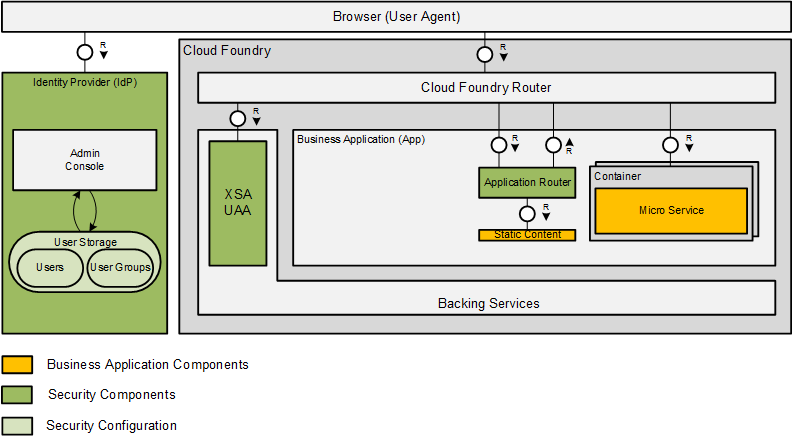
\includegraphics[width=1\textwidth]{../Security/images/XSA-Overview-Authentication}}
\end{frame}

% * . . . Authentication - IdP and UAA . . . *
\begin{frame}{Authentication - IdP and UAA}

\begin{columns}
    \begin{column}[T]{.47\textwidth}
    \textbf{SAML 2 IdP: Identity Provider}
    \begin{itemize}
        \item Authenticates Business Users
        \item Manages User Data and User Groups
        \item Issues SAML 2 Assertions about a Users Identity and Assigned User Groups
    \end{itemize}
    \end{column}
    \begin{column}[T]{.53\textwidth}
    \textbf{XS-UAA: User Account \& Authentication}
    \begin{itemize}
        \item Issues  Authorization Codes and JWT Tokens
%        \item Acts as OAuth 2.0 Server 
%        \item Maps User Groups to App's Authorization Model %Maps User Accounts to Authorizations of Business Apps
    \end{itemize}
    \end{column}
\end{columns}
\vfill
\begin{itemize}
\item UAA and IdP have a trusted relationship
\item XS-UAA is provided as backing service on SAP CP Cloud Foundry
\end{itemize}
\end{frame}


\begin{frame}{Authentication - Application Router}{Reverse Proxy}
\textbf{One \colorlink{https://wiki.wdf.sap.corp/wiki/download/attachments/1815947157/Approuter-Bluebook.docx}{Application Router} for each Business Application}
	\begin{itemize}
		\item Node.JS application for central user authentication \newline and session management
		\item Provides a \emph{\textbf{single entry point}} for the application 
		      \\- satisfies the \colorlink{https://en.wikipedia.org/wiki/Same-origin_policy}{Same Origin Policy}, \ldots
		\item Serves static content and forwards user requests to apps
	\end{itemize}
\vfill
\centerline{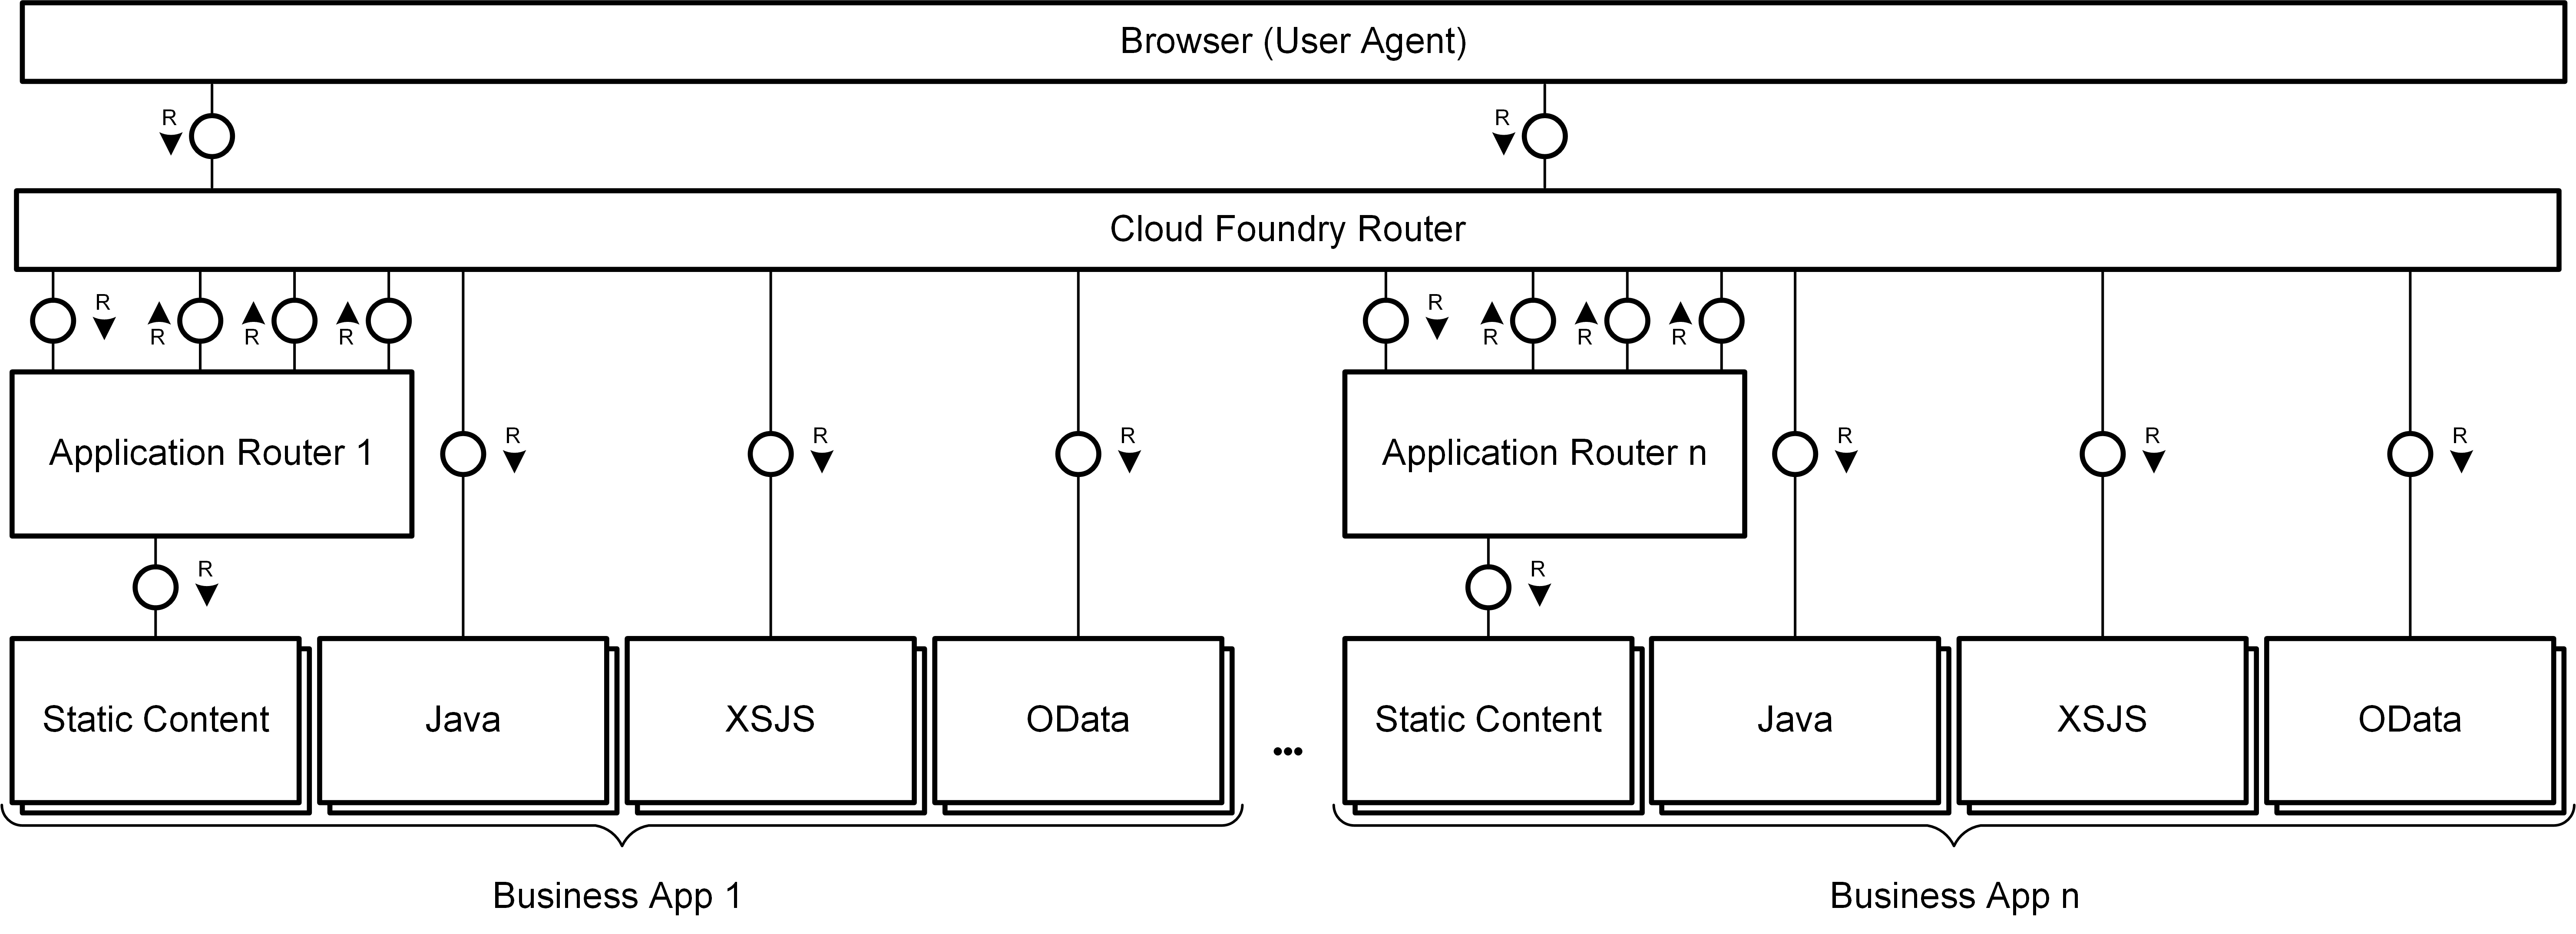
\includegraphics[width=0.9\textwidth]{../Security/images/ApplicationRouter}}
\end{frame}


\begin{frame}{Authentication Flow}{SAML 2 Authentication with OAuth 2.0 Authorization Code Grant}
\centerline{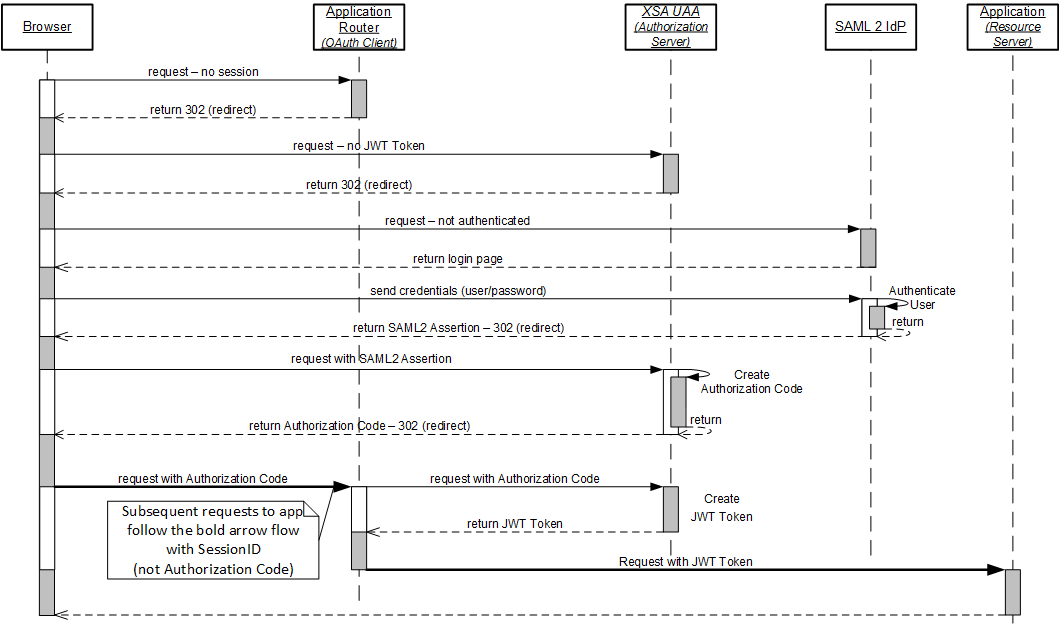
\includegraphics[width=1\textwidth]{../Security/images/OAuth2Flow}}
\end{frame}


\begin{frame}[fragile,t]{Setup Authentication - Configure Application Router}
\colorlink{https://github.wdf.sap.corp/xs2/approuter.js}{Application Router} provides URL rewriting
\begin{block}{Content of \codealt{./approuter/xs-app.json}}
\vspace{-3mm}
\scriptsize
\begin{lstlisting}[style=json]
{   "routes": [{
        "source": "^/ads",
        "target": "/",
        "destination": "ads-destination" }]
}
\end{lstlisting}
\vspace{-5mm}
\end{block}
\vfill
\begin{block}{Additional content of \codealt{manifest.yml}}
\vspace{-3mm}
\scriptsize
       \begin{verbatim}
- name: approuter
  env:
    TENANT_HOST_PATTERN: "^(.*)-bulletinboard-ads.cfapps.sap.hana.ondemand.com
    destinations: >
      [{ "name":"ads-destination", 
         "url":"https://bulletinboard-ads.cfapps.sap.hana.ondemand.com",
         "forwardAuthToken": true}]
  services:
    - uaa-bulletinboard
\end{verbatim}
\vspace{-5mm}
\end{block}
\end{frame}


\begin{frame}[fragile,t]{Excursion: JSON Web Token (JWT)}
Represents claims securely between two parties, \ldots
\scriptsize
\begin{lstlisting}[style=json]
{
  "client_id": "sb-bulletinboard-d012345!t1928",
  "iss": "http://localhost:8080/uaa/oauth/token",
  "exp": 1453498324,
  "scope": [
    "bulletinboard!t27.Display"
  ],
  "user_name": "anyUser@email.com",
  "user_id": "b07aaaf8-e704-4080-84cf-aae788162837",  
  "zid": "a09a3440-1da8-4082-a89c-3cce186a9b6c"
}
\end{lstlisting}
\vfill
\begin{itemize}
\item Token has maximum size (16 KB) -  don't make app's Authorization Model too complex!
\item UAA Service signs token with private key, \\public key is provided as part of \codealt{VCAP\_SERVICES} (verificationkey)
\item Tenant Id is provided in \codealt{zid} (Identity Zone)
\item \colorlink{https://jwt.io/introduction}{Introduction to JSON Web Tokens}
\end{itemize}
\end{frame}


\begin{frame}{Exercise 22}
	\begin{figure}
		\includeGraphicsExerciseTwentyTwo{width=0.9\textwidth}
	\end{figure}
\colorlink{https://github.wdf.sap.corp/cc-java-dev/cc-coursematerial/blob/master/Security/Exercise_22_DeployApplicationRouter.md}{Exercise 22: Deploy Application Router}
\end{frame}


\begin{frame}{Generic Authorizations}{Defining Authorizations for Endpoint Access}
\centerline{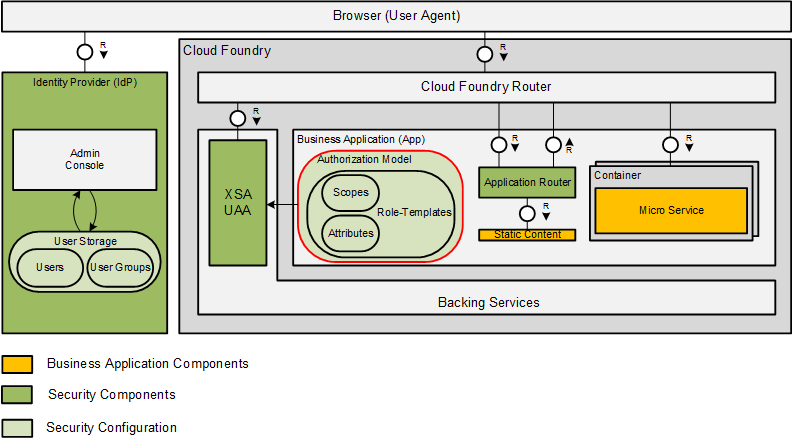
\includegraphics[width=1\textwidth]{../Security/images/XSA-Overview-Authorization}}
\end{frame}


\begin{frame}[fragile,t]{Define Application Authorization Model}
\colorlink{http://hanaxsdev.mo.sap.corp:8025/sap/hana/xs/docs/deploy_guide/default.html?df31a08a2c164520bb7e558103dd5adf.html}{Create Security Descriptor} for your application:
\begin{block}{Content of \codealt{./security/xs-security.json}}
\vspace{-3mm}
	\tiny
	\begin{lstlisting}[style=json]
{ "xsappname" : "bulletinboard-d012345",
  "tenant-mode" : "shared"
  "scopes" : [
              { "name" : "$XSAPPNAME.Display", "description" : "" },
              { "name" : "$XSAPPNAME.Update", "description" : "" }],
  "attributes" : [
              { "name" : "costcenter", "description" : "", "valueType" : "string" }],
  "role-templates" : [
              { "name" : "Viewer", "description" : "read only",
                          "scope-references" : [ "$XSAPPNAME.Display" ],
                          "attribute-references" : [ "costcenter" ]},
              { "name" : "Advertiser", "description" : "crud", 
                          "scope-references" : [ "$XSAPPNAME.Display", "$XSAPPNAME.Update" ],
                          "attribute-references": [ "costcenter" ]}
              ]}
}
	\end{lstlisting}
	\vspace{-5mm}
\end{block}
\vfill
Configure XSA UAA service instance with security descriptor
\scriptsize
\begin{lstlisting}
cf update-service uaa-bulletinboard -c security/xs-security.json
\end{lstlisting}
\end{frame}


\begin{frame}[fragile]{Define Generic Authorization Checks}
	Application Router restricts access based on scopes (start condition)
	\vspace{-2mm}
    \begin{block}{Additional content in \codealt{./approuter/xs-app.json}}
		\vspace{-3mm}
		\scriptsize
	\begin{lstlisting}[style=json]
{	"routes": [{
    "source": "^/ads",
    "target": "/",
    "destination": "ads-destination",
    "scope": "$XSAPPNAME.Display"         # <-- new
    }]
}
		\end{lstlisting}
		\vspace{-5mm}
	\end{block}
\end{frame}


\begin{frame}{Exercise 23}
	\colorlink{https://github.wdf.sap.corp/cc-java-dev/cc-coursematerial/blob/master/Security/Exercise_23_SetupGenericAuthorization.md}{Exercise 23: Setup Generic Authorization}
\end{frame}


\begin{frame}{Domain specific Authorizations}{Defining Authorizations for Business Functions}
\centerline{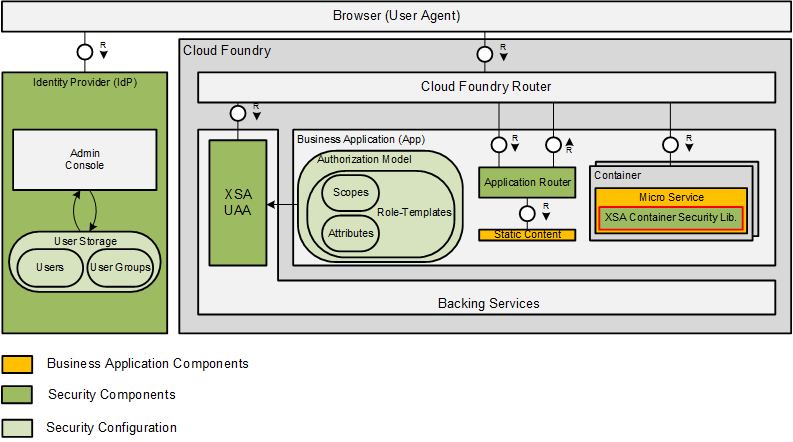
\includegraphics[width=1\textwidth]{../Security/images/XSA-Overview-All}}
\end{frame}

\begin{frame}[fragile,t]{SAP Java Container Security library} {based on Spring Security}

Spring Security and Spring Security OAuth
\begin{itemize}
	\item ensures that application calls are authenticated \& authorized
	\item enablement through Servlet Filter chain (\colorlink{http://docs.spring.io/autorepo/docs/spring-security/3.2.5.RELEASE/apidocs/org/springframework/security/web/context/AbstractSecurityWebApplicationInitializer.html}{Example})
	\item supports offline JWT token validation
	\item \ldots
\end{itemize}
\vfill
\colorlink{http://nexusrel.wdf.sap.corp:8081/nexus/\#nexus-search;quick\%7Ejava-container-security}{SAP Container Security library}
\begin{itemize}
	\item extends Spring Security \& Spring Security OAuth
	\item allows domain specific authorization checks \\e.g. "Change Cost Center"
	\item implements offline JWT token validation
\end{itemize}
% add picture to explain offlineToken, DelegatingFilterProxy, ..
\end{frame}



\begin{frame}[fragile,t]{Spring Security}{Register Spring Security Filter-Chain}
\scriptsize
\begin{lstlisting}[language=java]
public class AppInitializer implements WebApplicationInitializer {
...
  @Override
    public void onStartup(ServletContext servletContext) throws ServletException {
    ...
    // register Spring Security Filter-Chain
    servletContext
      .addFilter(AbstractSecurityWebApplicationInitializer.DEFAULT_FILTER_NAME,
        newDelegatingFilterProxy(AbstractSecurityWebApplicationInitializer
          .DEFAULT_FILTER_NAME))
      .addMappingForUrlPatterns(EnumSet.allOf(DispatcherType.class), false, "/*");
    ...
  }
  ...
}
\end{lstlisting} 
\end{frame}

\begin{frame}[fragile,t]{Spring Security}{Configure Authorizations}
\scriptsize
\begin{lstlisting}[language=java]
@Configuration
@EnableWebSecurity
public class SecurityConfig extends ResourceServerConfigurerAdapter {
	@Override
	public void configure(HttpSecurity http) throws Exception {
       http
          .sessionManagement()
               .sessionCreationPolicy(SessionCreationPolicy.NEVER)
               .and().authorizeRequests()
          /* from specific to generic url */          
          .antMatchers(HttpMethod.POST, "/api/v1/ads/**")
               .access("#oauth2.hasScope('bulletinboard.Update')")
		  .antMatchers(GET, "/", "/health").permitAll() //accepts not-auth users
          .anyRequest().denyAll();
     }
\end{lstlisting} 
\begin{itemize}
	\item \codealt{@EnableWebSecurity} defines Spring Security configuration
	(similar to \codealt{security.xml}). \\\colorlink{https://github.wdf.sap.corp/cc-java/cc-bulletinboard-ads-spring-webmvc/blob/solution-24-Make-App-Secure/src/main/java/com/sap/bulletinboard/ads/config/WebSecurityConfig.java}{Example Configuration}
\end{itemize}
\end{frame}

\begin{frame}[t]{Extract of the SAP Container Security Library}
\textbf{SecurityContext.getUserInfo() : UserInfo}
	\begin{itemize}
		\item \scriptsize Static Method - Returns an object of type \textbf{UserInfo}
	\end{itemize}
		\textbf{userInfo.checkLocalScope(String scopeName) : Boolean}
	\begin{itemize}
		\item  \scriptsize Checks a scope of the current application - scope without prefix
	\end{itemize}
\textbf{userInfo.checkScope(String scopeName) : Boolean}
	\begin{itemize}
		\item  \scriptsize Checks a scope of an external application - scope prefixed by application name
	\end{itemize}
\textbf{userInfo.getAttribute(String attributeName) : String[]}
	\begin{itemize}
		\item  \scriptsize Returns attribute values (e.g. Cost Center) passed from authentication
	\end{itemize}
\textbf{userInfo.getIdentityZone() : String}
	\begin{itemize}
		\item  \scriptsize Returns identity zone which is equal to the \textbf{tenant ID}
	\end{itemize}
\textbf{userInfo.getDBToken() : String}
	\begin{itemize}
		\item  \scriptsize Get a personalized DB access token for connecting to the HANA DB
	\end{itemize}
\end{frame}


\begin{frame}[fragile,t]{Alternative Authentication Check}
\vspace{-3mm}
\begin{lstlisting}[language=java]
    public User() {
        userInfo = getUserInfo();
    }

    private UserInfo getUserInfo() {
        try {
            return SecurityContext.getUserInfo();
        } catch (UserInfoException e) {
            logger.error("User not authenticated", e);
            throw new NotAuthorizedException(e); // 401 HTTP Status Code
        }
    }
\end{lstlisting}
\begin{itemize}
	\item Default message of \codealt{NotAuthorizedException} is misleading. \\Needs to be "not authenticated"
\end{itemize}
\end{frame}


\begin{frame}[fragile,t]{Domain specific Authorization Check}
\vspace{-3mm}
\begin{lstlisting}[language=java]
    public void throwIfNotAuthorizedForLocalScope(String scope) {
        if (!isAuthorizedForLocalScope(scope)) {
            logger.error("User not authorized for local scope: {}", scope);
            throw new ForbiddenException(); // 403 HTTP Status Code
        }
    }

    public boolean isAuthorizedForLocalScope(String scope) {
        try {
            return userInfo.checkLocalScope(scope);
        } catch (UserInfoException e) {
            logger.error("Method UserInfo.checkLocalScope for scope {} failed", scope, e);
            throw new ServerErrorException(HttpStatus.SC_INTERNAL_SERVER_ERROR, e);
        }
    }
\end{lstlisting}
\vspace{-5mm}
\end{frame}


\begin{frame}[fragile,t]{Obtaining Information about the Current User}
\begin{lstlisting}[language=java]
try {
    logonName = userInfo.getLogonName();
    email = userInfo.getEmail();
    givenName = userInfo.getJsonValue("givenName");
    familyName = userInfo.getJsonValue("familyName");
} catch (UserInfoException e) {
    // handle exception
}
\end{lstlisting}
\colorlink{https://github.wdf.sap.corp/xs2-samples/java-hello-world}{Example - Java Hello World}
\end{frame}


\begin{frame}{Exercise 24}
    \begin{figure}
        \includeGraphicsExerciseTwentyFour{width=0.8\textwidth}
    \end{figure}
\colorlink{https://github.wdf.sap.corp/cc-java-dev/cc-coursematerial/blob/master/Security/Exercise_24_MakeYourApplicationSecure.md}{Exercise 24: Make Application Secure}
\end{frame}


\begin{frame}{Data Model of Authentication and Authorization}
\centerline{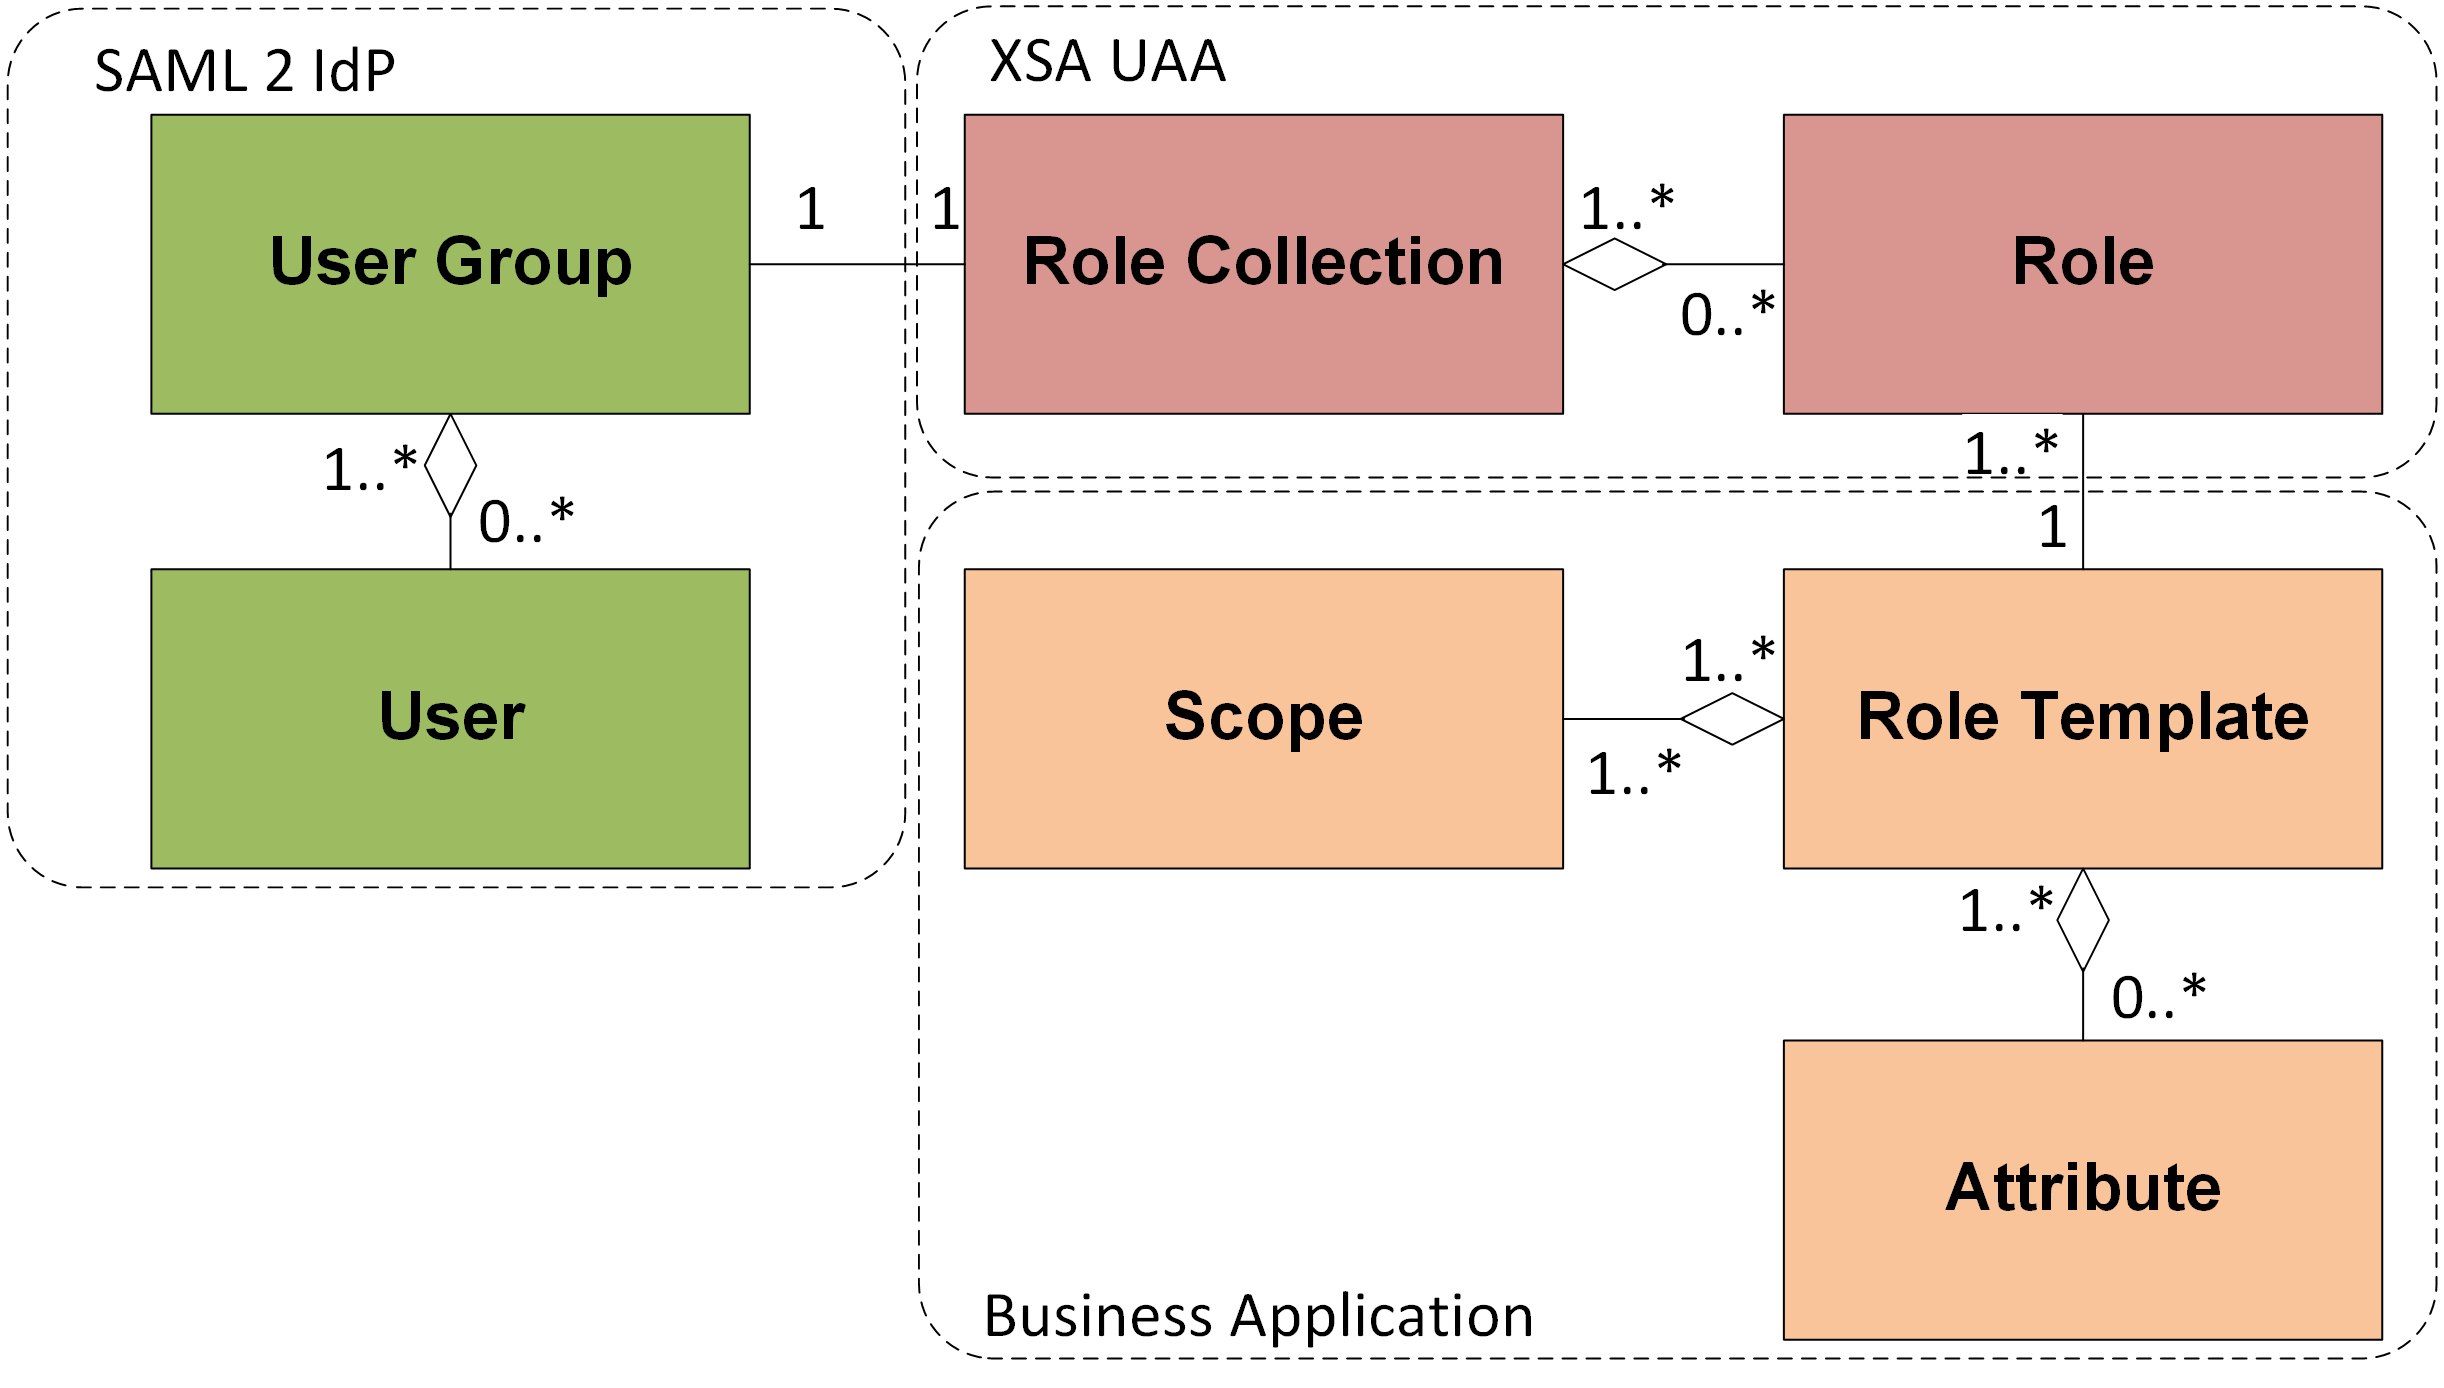
\includegraphics[width=\textwidth]{../Security/images/ERRolesAndScopes}}
\vfill
\scriptsize
Depending on IdP configuration: Role Collection is mapped directly to User OR to User Group
\end{frame}


\begin{frame}[t]{SAP CP Cockpit - Security}{Create Role-Collection and assign Role(s)}
\centerline{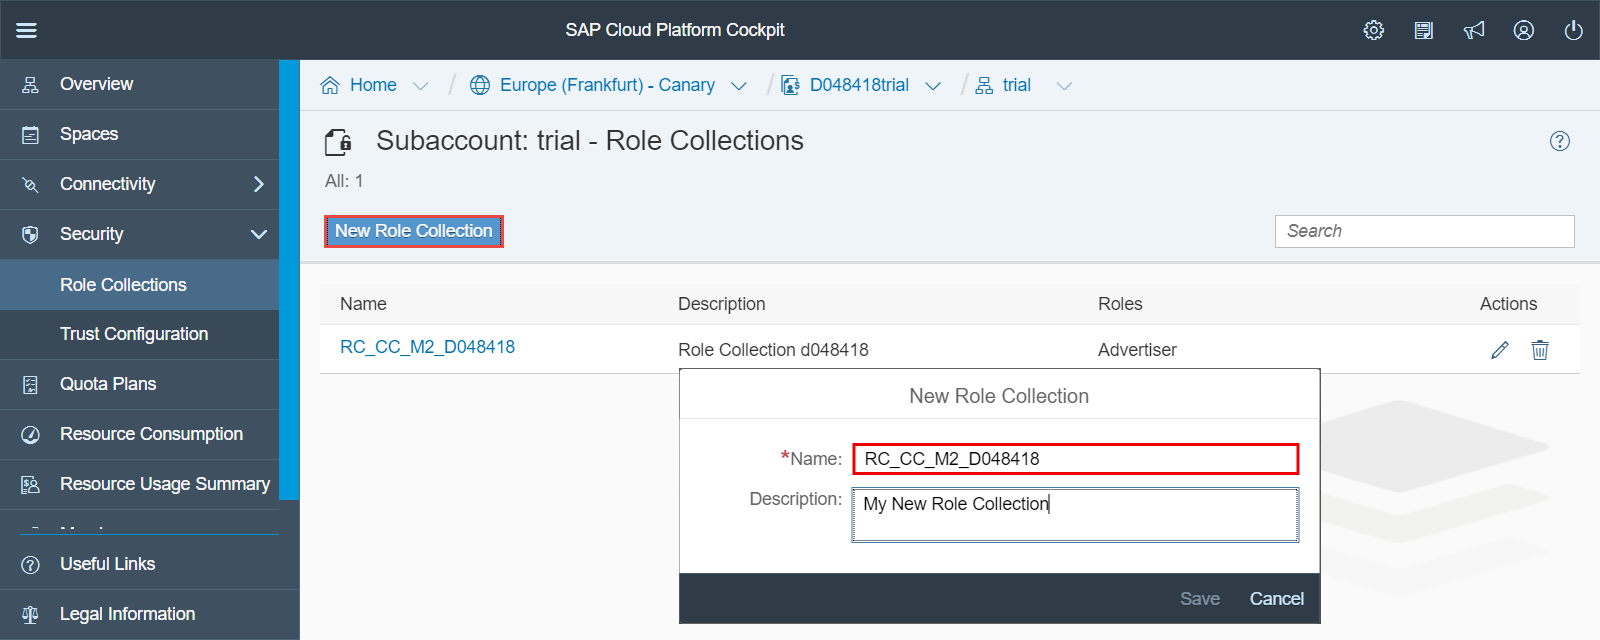
\includegraphics[width=\textwidth]{../Security/images/CockpitRoleCollectionCreate}}
\scriptsize
\vfill
Note: Roles can be explicitly defined in context of your application \colorlink{https://jam4.sapjam.com/wiki/show/d2dgJlWR9IpwQsLOCmyJj9?_lightbox=true}{How to}.
\end{frame}

\begin{frame}[t]{SAP CP Cockpit - Security}{Create Role-Collection and assign Role(s)}
\centerline{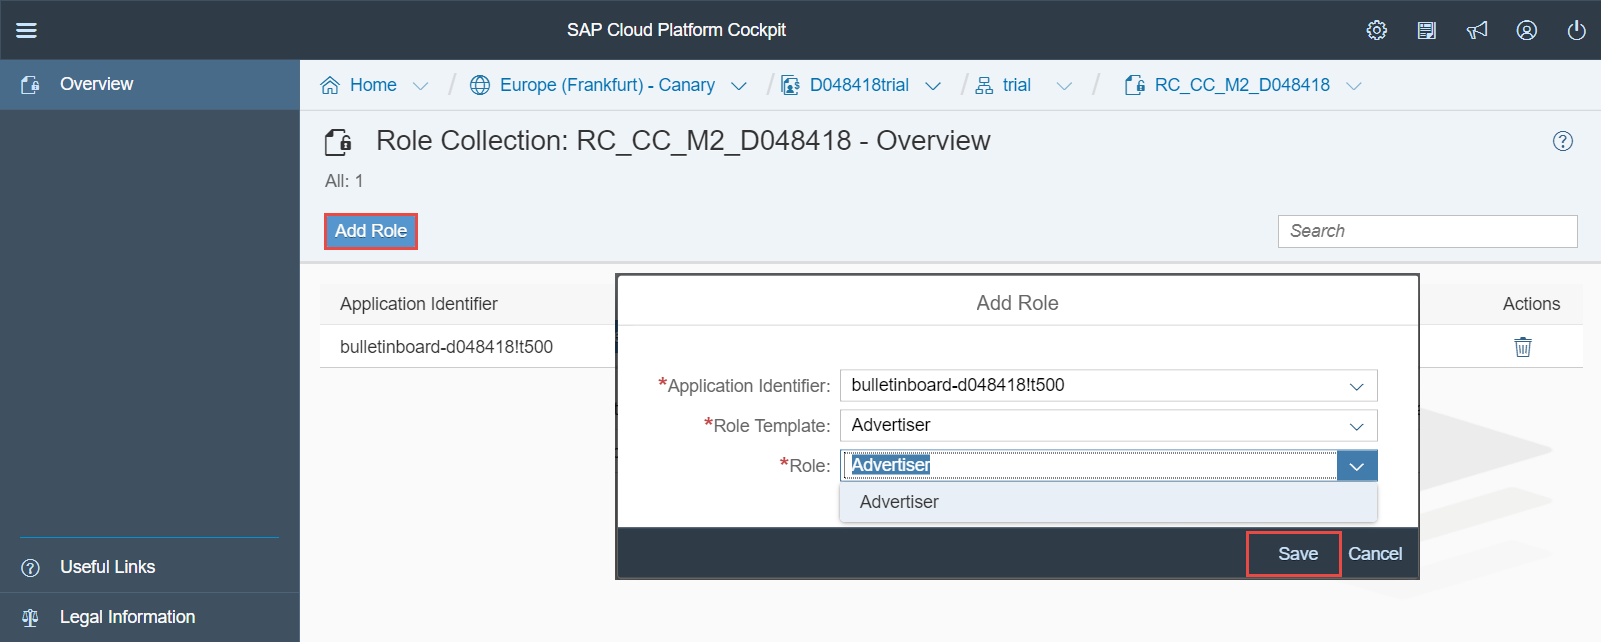
\includegraphics[width=\textwidth]{../Security/images/CockpitRoleCollectionAddRole}}
\end{frame}

\begin{frame}[t]{SAP CP Cockpit - Security}{Assign Role Collection to User}
\centerline{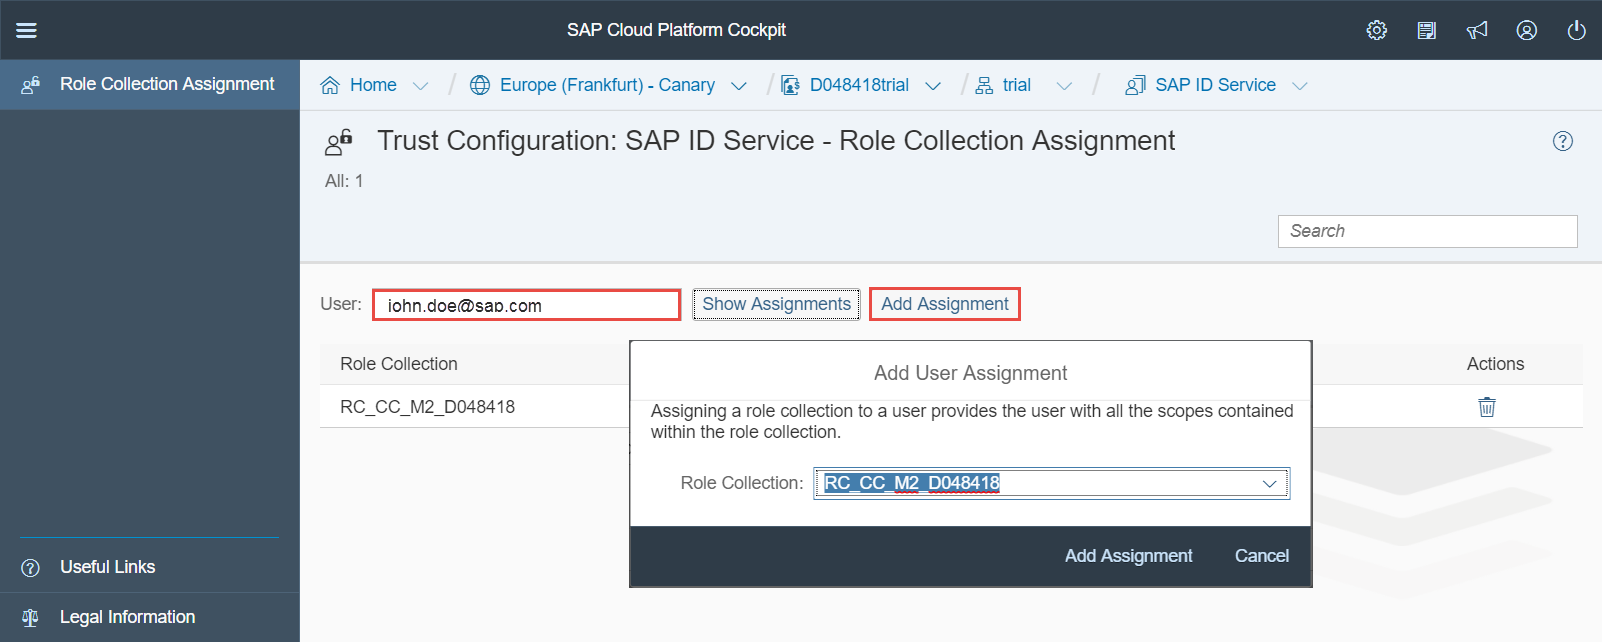
\includegraphics[width=\textwidth]{../Security/images/CockpitRoleCollectionAssignToUser}}
\vfill
\scriptsize
Prerequisite: User needs to log in to the subaccount at least once e.g. 
\\\colorlink{https://d012345trial.authentication.sap.hana.ondemand.com}{https://d012345trial.authentication.sap.hana.ondemand.com}\\
\vfill
Authorizations assigned to your User? Check via 
\\\colorlink{https://d012345trial.authentication.sap.hana.ondemand.com/config?action=who}{https://d012345trial.authentication.sap.hana.ondemand.com/config?action=who}
\end{frame}

\begin{frame}[t]{SAP CP Cockpit - Security}{Configure Trust to Fake IdP (Muenchhausen)}
\centerline{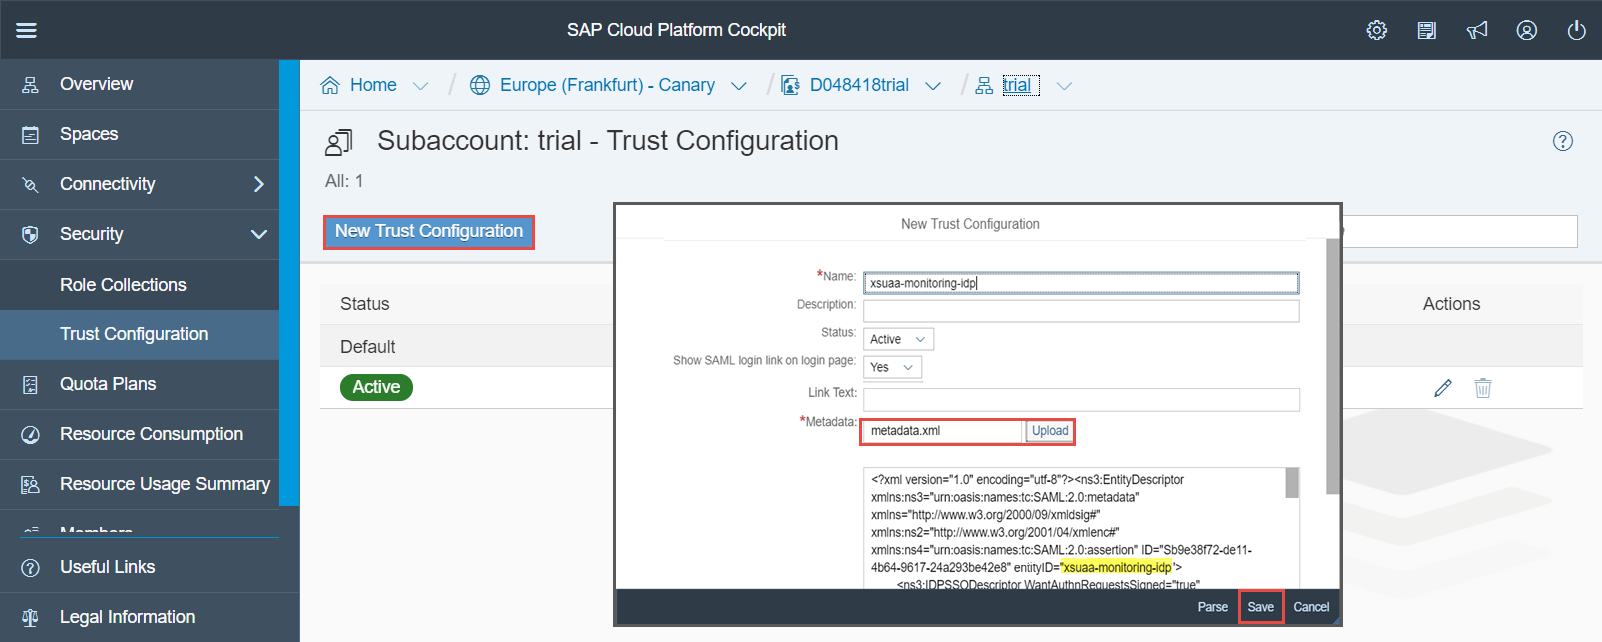
\includegraphics[width=\textwidth]{../Security/images/AddMuenchhausenFakeIdP}}
\vfill
\scriptsize
You can get the \textit{metadata.xml} from Muenchhausen via \colorlink{https://xsuaa-monitoring-idp.cfapps.sap.hana.ondemand.com/saml/metadata}{https://xsuaa-monitoring-idp.cfapps.sap.hana.ondemand.com/saml/metadata}
\end{frame}


\begin{frame}[t]{Requirements for Productive Applications}
	\begin{itemize}
		\item \textbf{DO} ensure that the Jot-Token (JWT) is provided by the request
		\item \textbf{DO} define scopes for generic authorization checks in \codealt{xs-app.json}
		\item \textbf{DO} define scopes for domain authorization checks in \codealt{xs-security.json}
		\item \textbf{DO} \colorlink{https://github.wdf.sap.corp/xs2/approuter.js/blob/v2.6.1/README.md\#central-logout}{support logout functionality} in your UIs
		\item \textbf{DO NOT} trace Jot-Tokens (JWTs)
	\end{itemize}
\end{frame}


\begin{frame}[t]{Further Information}
	\begin{itemize}
		\item \colorlink{https://github.wdf.sap.corp/cc-java-dev/cc-coursematerial/blob/master/Security/Readme.md}{Security Detail Notes - e.g. Service to Service Communication}
		\item \colorlink{https://jam4.sapjam.com/groups/DRuoC97ApSanbbXx20g4kb/forums?folder_id=AMNslm97NHCbh0z28jNy7D}{XS Security JAM Forum}
		\item \colorlink{https://wiki.wdf.sap.corp/wiki/display/xs2/Security}{SAP Wiki - XS2 - Security}
		\item \colorlink{https://github.wdf.sap.corp/xs2/xs2-docs/wiki/SecurityLibrary}{SAP GitHub - XS2 Docs Wiki - Security Library}
		\item \colorlink{https://sap.plateau.com/learning/user/deeplink_redirect.jsp?linkId=ITEM_DETAILS&componentID=70242962&componentTypeID=COURSE&revisionDate=1404129600000&fromSF=Y&company=SAP}{E-Learning - Threat Modeling Methodology}
		\item \colorlink{https://sap.plateau.com/learning/user/deeplink_redirect.jsp?linkId=ITEM_DETAILS&componentID=70261541&componentTypeID=COURSE&revisionDate=1404129600000&fromSF=Y&company=SAP}{Classroom - Threat Modeling Methodology}
		\item \colorlink{https://sap.plateau.com/learning/user/deeplink_redirect.jsp?linkId=ITEM_DETAILS&componentID=70226407&componentTypeID=COURSE&revisionDate=1404129600000&fromSF=Y&company=SAP}{E-Learning - Secure Programming for Java}
		\item \colorlink{https://jam4.sapjam.com/groups/hwsYB62safobfg6sX9QrYW/overview_page/43624}{E-Learning - Fortify Online Training}
		\item \colorlink{https://sap.plateau.com/learning/user/deeplink_redirect.jsp?linkId=ITEM_DETAILS&componentID=70226408&componentTypeID=COURSE&revisionDate=1404129600000&fromSF=Y&company=SAP}{E-Learning - Product Security Awareness}
	\end{itemize}
\end{frame}
